\documentclass[12pt,a4paper]{article}
\usepackage[utf8]{inputenc}
\usepackage[italian]{babel}
\usepackage[T1]{fontenc}
\usepackage{lmodern} % O usa 'times' per un font più simile al PDF
\usepackage{geometry}
\geometry{margin=3cm}
\usepackage{graphicx}
\usepackage{fancyhdr}
\usepackage{setspace}
\usepackage{titlesec}
\usepackage{caption}
\usepackage{booktabs}
\usepackage{float}
\usepackage{hyperref}
\usepackage{array}
\usepackage{listings}

\usepackage{listings}
\usepackage{xcolor}

\lstdefinelanguage{SQL}{
    morekeywords={SELECT, FROM, WHERE, AND, OR, INSERT, INTO, VALUES, UPDATE, SET, DELETE, CREATE, TABLE, ALTER, DROP, JOIN, ON, AS, IN, IS, NOT, NULL, LIKE, DISTINCT, ORDER, BY, GROUP, HAVING, LIMIT},
    sensitive=false,
    morecomment=[l]--,
    morestring=[b]',
}

\lstset{
    language=SQL,
    basicstyle=\ttfamily\small,
    keywordstyle=\color{violet}\bfseries,
    commentstyle=\color{gray},
    stringstyle=\color{orange},
    backgroundcolor=\color{white},
    showstringspaces=false,
    breaklines=true,
    captionpos=b
}

\graphicspath{ {./images/} }
\pagestyle{plain}
\onehalfspacing % Interlinea 1.5
\setlength{\parskip}{0.5em}

% ------------------ FRONTESPIZIO ------------------
\begin{document}
\begin{titlepage}
    \centering
    {\scshape\LARGE Università degli Studi di Padova \par}
    \vspace{1cm}
    {\scshape\Large Corso di Laurea in Informatica \par}
    \vspace{3cm}
    {\Huge\bfseries Base di Dati per un Sistema di gestione di Serie TV in Streaming \par}
    \vspace{2cm}
    {\Large Gruppo: Ceron Tommaso, Parolin Dennis\par}
    \vfill
    {\large Anno Accademico 2024/2025\par}
\end{titlepage}

------------------ INDICE  ------------------
\tableofcontents
\newpage

% ------------------ CONTENUTO ------------------

\section{Abstract}
Questo progetto sviluppa una base di dati per gestire delle serie tv, composte da stagioni ed episodi, e dai loro attori e registi. Inoltre, questa base di dati permette di gestire degli utenti e gli episodi che guardano, ai quali possono dare un voto.\newline L'obbiettivo principale è quello di gestire la struttura delle serie tv, gestire le relazioni di quest’ ultime con il cast e il regista che vi partecipa e infine registrare ciò che un utente guarda.\newline
La base di dati distingue le persone in utenti, registi e attori, ognuno con degli attributi e relazioni distinte.\newline
Una serie si compone di almeno una stagione, che a sua volta è composta da almeno un episodio. Opzionalmente una Serie TV può anche contenere una Opening (ovvero una sigla iniziale).\newline
Infine, il sistema tiene traccia delle piattaforme di streaming che mettono a disposizione una determinata serie tv, e degli utenti che sottoscrivono un abbonamento con uno o più di queste piattaforme. \newline

\section{Analisi dei Requisiti}
In questa sezione riassumiamo i requisiti che caratterizzano la base di dati.\newline\newline
\textbf{Serie TV.} Una serie TV è identificata da un titolo e un anno e contiene questi attributi:
\begin{itemize}
  \item Titolo
  \item Anno di Inizio
  \item Descrizione
  \item Genere
\end{itemize}
Una Serie TV è composta da una o più stagioni, e da zero o una Opening (sigla iniziale) \newline\newline\newline\newline
\textbf{Stagioni.} Una stagione è identificata dal suo numero e dalla Serie Tv a cui appartiene, e contiene questi attributi:
\begin{itemize}
    \item Numero
    \item Anno
\end{itemize}
Una stagione è composta da uno o più episodi\newline\newline
\textbf{Episodio.} Un episodio è identificato dal suo numero e dalla stagione a cui appartiene, e contiene questi attributi:
\begin{itemize}
    \item Numero
    \item Durata (in minuti)
    \item Titolo
    \item Numero di utenti (che hanno guardato l' episodio)
\end{itemize}
\textbf{Opening.} Una opening è identificata da un titolo, e contiene questi attributi:
\begin{itemize}
    \item Titolo
    \item Compositore
    \item Durata
\end{itemize}
\textbf{Persona.} Una persona generica è identificata da un codice fiscale e contiene i seguenti attributi: 
\begin{itemize}
    \item Codice Fiscale
    \item Nome
    \item Data di nascita
\end{itemize}
Una persona si suddivide in \textbf{Utente}, \textbf{Nome} e \textbf{Registi}\newpage
\textbf{Utenti.} Un utente, oltre agli attributi di \textit{Persona} contiene:
\begin{itemize}
    \item Username
    \item Email
\end{itemize}
\textbf{Attore.} Un attore, oltre agli attributi di \textit{Persona}, contiene:
\begin{itemize}
    \item Nazionalita'
    \item Il numero di film in cui ha partecipato
\end{itemize}
\textbf{Regista.} Un regista, oltre agli attributi di \textit{Persona}, contiene:
\begin{itemize}
    \item Nazionalita
    \item Il genere di film creati
\end{itemize}
\textbf{Piattaforma streaming.} Una piattaforma streaming e' identificata dal suo nome e contiene i seguenti attributi:
\begin{itemize}
    \item Nome 
    \item Costo mensile
\end{itemize}
\section{Progettazione concettuale}
\subsection{Lista entità}
Il database si compone delle seguenti entità:
\begin{itemize}
    \item \textbf{SerieTV:} Rappresenta una Serie Tv univoca, con una o più stagioni.
    \begin{itemize}
        \item \underline{Titolo}: string
        \item \underline{AnnoInizio} (ovvero l'anno della prima stagione): int
        \item Genere: string
        \item Descrizione: string
    \end{itemize}
    \item \textbf{Stagione:} Rappresenta una stagione di una specifica Serie Tv
    \begin{itemize}
        \item \underline{Numero\_stagione}: int
        \item Anno: int
    \end{itemize}
    \item \textbf{Episodio:} Rappresenta un singolo episodio di una specifica stagione
    \begin{itemize}
        \item \underline{Numero\_episodio}: int
        \item Durata (in minuti): int
        \item Titolo: string
        \item Numero\_utenti (che hanno guardato l'episodio): int
    \end{itemize}
    \item \textbf{Opening:} Rappresenta la sigla iniziale di una SerieTv, se presente.
    \begin{itemize}
        \item \underline{Titolo}: string
        \item Durata: int
        \item Compositore: string
    \end{itemize}
    \item \textbf{Persona:} Rappresenta una persona generica.
    \begin{itemize}
        \item \underline{Codice Fiscale}: int
        \item Nome: string
        \item Data\_nascita: date
    \end{itemize}
    \item \textbf{Utente:} Rappresenta una specializzazione di Persona, rappresenta un abbonato a una o più piattaforme streaming
    \begin{itemize}
        \item Username: string
        \item Email: string
    \end{itemize}
    \item \textbf{Attore:} Rappresenta una specializzazione di Persona, partecipa a una o più serie TV.
    \begin{itemize}
        \item Nazionalità: string
        \item Numero\_serie (in cui ha partecipato): int
    \end{itemize}
    \item \textbf{Regista:} Rappresenta una specializzazione di Persona, ha diretto una o più serie TV.
    \begin{itemize}
        \item Nazionalita: string
        \item Genere\_serie: string
    \end{itemize}
    \item \textbf{Piattaforma streaming:} Rappresenta una piattaforma che contiene una o più serie Tv, e a cui gli utenti possono abbonarsi con vari tipi di abbonamento.
    \begin{itemize}
        \item \underline{Nome}: string
        \item Costo\_mensile: float
    \end{itemize}
\end{itemize}
\subsection{Lista relazioni}
\begin{itemize}
    \item Serie TV$\Rightarrow$(1, N)$\Rightarrow$ComposizioneStag$\Leftarrow$(1,1)$\Leftarrow$Stagione 
    \begin{itemize}
        \item Una Serie Tv è composta da una o più stagioni
        \item Una stagione compone una sola Serie Tv 
    \end{itemize}
    \item Stagione$\Rightarrow$(1, N)$\Rightarrow$ComposizioneEP$\Leftarrow$(1,1)$\Leftarrow$Episodio
    \begin{itemize}
        \item Una stagione è composta da uno o più episodi
        \item Un episodio compone una sola stagione
    \end{itemize}
    \item Serie TV$\Rightarrow$(1,1)$\Rightarrow$Contenimento$\Leftarrow$(1, N)$\Leftarrow$Piattaforma-Streaming
    \begin{itemize}
        \item Una Serie Tv è contenuta (può essere vista) in una sola piattaforma streaming
        \item Una piattaforma streaming può contenere una o più serie tv 
    \end{itemize}
    \item Piattaforma-Streaming$\Rightarrow$(1, N)$\Rightarrow$Sottoscrizione$\Leftarrow$(1, N)$\Leftarrow$Utente
    \begin{itemize}
        \item Ad una piattaforma streaming si sottoscrivono uno o più utenti
        \item Un utente può sottoscriversi a una o più piattaforme streaming (minimo una per essere considerato utente)
        \item Questa relazione contiene i seguenti attributi:
        \begin{itemize}
            \item Data\_inizio: date
            \item Data\_fine: date
            \item Tpo\_abbonamento: string
        \end{itemize}
    \end{itemize}\newpage
    \item Utente$\Rightarrow$(0, N)$\Rightarrow$Visiona$\Leftarrow$(0, N)$\Leftarrow$Episodio
    \begin{itemize}
        \item Un utente può vedere 0 o più episodi di stagioni differenti
        \item Un episodio generico può essere visto da nessuno o da più utenti
        \item Questa relazione contiene i seguenti attributi:
        \begin{itemize}
            \item Data: date
            \item Voto: int
        \end{itemize}
        Il voto è opzionale.
    \end{itemize}
    \item Serie TV$\Rightarrow$(1, N)$\Rightarrow$Perfomance$\Leftarrow$(1, N)$\Leftarrow$Attore
    \begin{itemize}
            \item In una serie tv recitano uno o più attori
            \item Un attore può recitare in una o più serie tv
            \item Questa relazione contiene i seguenti attributi:
            \begin{itemize}
                \item Ruolo: string
                \item Compenso: int
        \end{itemize}
    \end{itemize}
    \item Serie TV$\Rightarrow$(1,1)$\Rightarrow$Direzione$\Leftarrow$(1, N)$\Leftarrow$Regista 
    \begin{itemize}
        \item Una serie tv è diretta da un solo regista 
        \item Un regista può dirigere una o più serie 
    \end{itemize}
    \item Serie Tv$\Rightarrow$(0,1)$\Rightarrow$ContenimentoOpening$\Leftarrow$(1,1)$\Leftarrow$Opening
    \begin{itemize}
        \item Una serie tv contiene zero o una opening
        \item Una opening appartiene a una sola Serie Tv 
    \end{itemize} 
\end{itemize}
\subsection{Lista generalizzazioni}
\textbf{Persona} è una generalizzazione totale di \textbf{UTENTE}, \textbf{ATTORE} e \textbf{REGISTA} 

\subsection{Schema E-R}
\textbf{In figura \ref{fig:no-ristrutt}} è riportato il diagramma E-R che riassume i requisiti discussi in precedenza.
\begin{figure}[h]
    \centering
    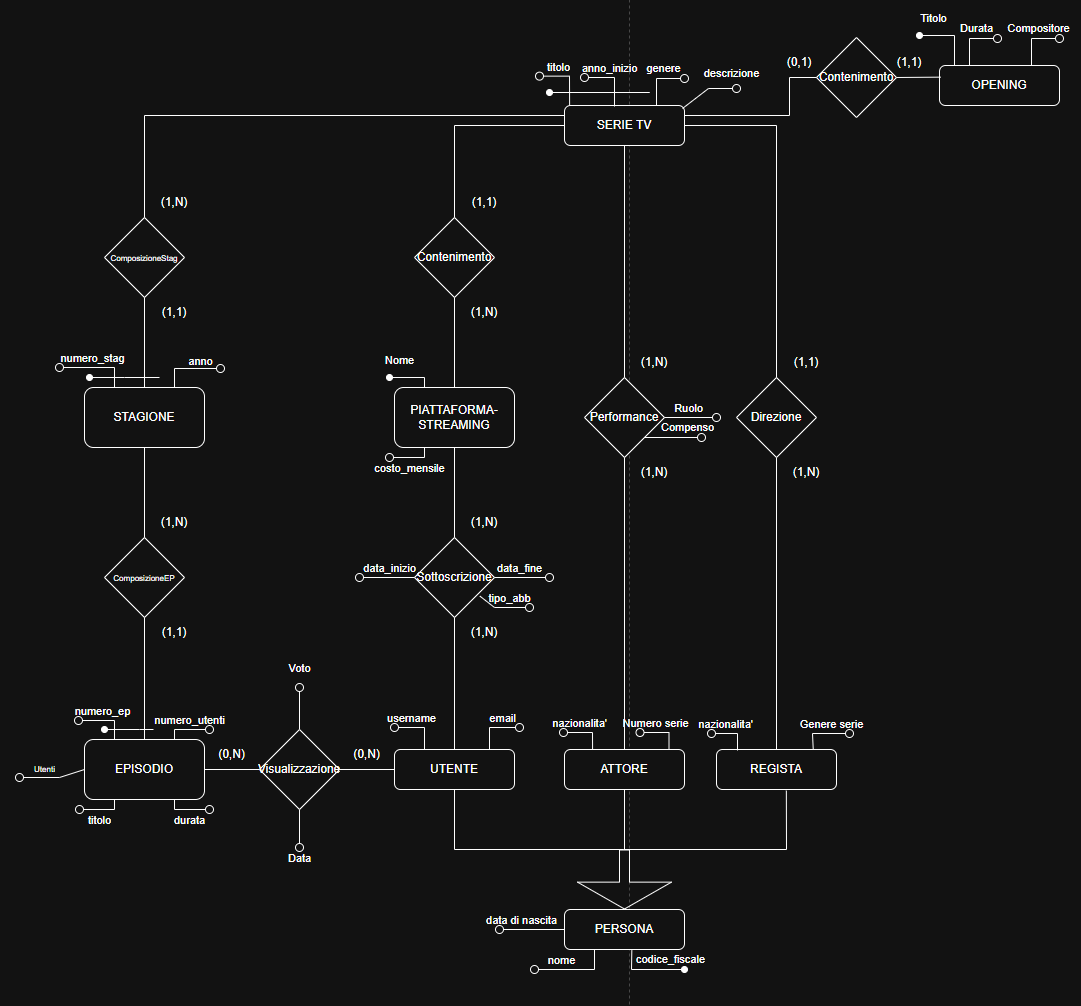
\includegraphics[scale=0.4]{schema-no-ristrutt.png}
    \caption{Schema E-R non ristrutturato}
    \label{fig:no-ristrutt}
\end{figure}
\section{Progettazione Logica}
In questa sezione illustriamo la traduzione dello schema concettuale in schema logico, per rappresentare i dati nel modo più efficace possibile. 
Andiamo quindi ad analizzare le ridondanze, per comprendere se sia preferibile eliminarle o mantenerle. 
Procediamo poi con l'eliminazione delle generalizzazioni e infine mostriamo lo schema ristrutturato.
\subsection{Analisi delle ridondanze}
\subsubsection{Ridondanza "NumeroSerieTv"}
Possiamo notare che attributo “Numero Serie Tv” del sottoinsieme “Attore” entità “Persona” può essere calcolato dalla relazione Perfomance, poiché è il conteggio di tutte le Serie Tv per quel determinato attore.
Questo attributo viene modificato (almeno una volta) ogni volta che viene inserita una nuova SerieTv (stimiamo circa 5 nuovi inserimenti al giorno)
e viene visualizzato ogni volta un utente vuole sapere in quanti film ha recitato un attore (stimiamo 25 al giorno).
Il tutto si riassume nelle seguenti operazioni:
\begin{itemize}
    \item \textbf{Operazione 1 (5 al giorno)}: inserimento di una nuova tupla in Perfomance
    \item \textbf{Operazione 2 (25 al giorno)}: Visualizzare in quanti film ha recitato un attore.
\end{itemize}

Assumiamo i seguenti dati:
\begin{center}
\begin{tabular}{|c c c|} 
 \hline
 Concetto & Costrutto & Volume \\ [0.5ex] 
 \hline\hline
 Attore & Entità  & 1000\\ 
 \hline
 Performance & Relazione & 2000\\[1ex] 
 \hline
\end{tabular}
\end{center}
\textbf{Con Ridondanza}
\begin{itemize}
    \item Operazione 1
    \begin{center}
    \begin{tabular}{|c|c|c|c|}
    \hline
    \textbf{Concetto} & \textbf{Costrutto} & \textbf{Accessi} & \textbf{Tipo} \\
    \hline
    Serie TV & E & 1 & S\rlap{\hspace{2.5em}$\times\,5$} \\
    Perfomance & R & 1 & S\rlap{\hspace{2.5em}$\times\,5$} \\
    Attore & E & 1 & L\rlap{\hspace{2.5em}$\times\,5$} \\
    Attore & E & 1 & S\rlap{\hspace{2.5em}$\times\,5$} \\
    \hline
    \end{tabular}
    \item Operazione 2
    \begin{center}
        \begin{tabular}{|c|c|c|c|}
        \hline
        \textbf{Conecetto} & \textbf{Costrutto} & \textbf{Accessi} & \textbf{Tipo} \\
        \hline
        Attore & E & 1 & L\rlap{\hspace{2.5em}$\times\,25$} \\
        \hline
        \end{tabular}
    \end{center}
    \end{center}
    Assumiamo costo doppio per le operazioni in scrittura, il costo totale ottenuto è:
    $((5\times 3)\times 2) + 5 + 25=60$
\end{itemize}
\textbf{Senza Ridondanza}
\begin{itemize}
    \item Operazione 1
    \begin{center}
        \begin{tabular}{|c|c|c|c|}
        \hline
        \textbf{Conecetto} & \textbf{Costrutto} & \textbf{Accessi} & \textbf{Tipo} \\
        \hline
        Serie Tv & E & 1 & S\rlap{\hspace{2.5em}$\times\,5$} \\
        \hline
        Performance & R & 1 & S\rlap{\hspace{2.5em}$\times\,5$} \\
        \hline
        \end{tabular}
    \end{center}
    \item Operazione 2\newline
    Stimiamo circa 2.000 performance attoriali
    \begin{center}
        \begin{tabular}{|c|c|c|c|}
        \hline
        \textbf{Conecetto} & \textbf{Costrutto} & \textbf{Accessi} & \textbf{Tipo} \\
        \hline
        Attore & E & 1 & L\rlap{\hspace{2.5em}$\times\,25$} \\
        \hline
        Performance & R & 2.000 & L\rlap{\hspace{2.5em}$\times\,25$} \\
        \hline
        \end{tabular}
    \end{center}
\end{itemize}
Assumiamo costo doppio per le operazioni in scrittura, il costo totale ottenuto è:
    $((5\times 2)\times 2)+25+(2000\times 25)\times 2=100.045$\newline
    Questo calcolo permette di stabilire che mantenere la ridondanza è preferibile,
    in modo da ottimizzare gli accessi.
\subsubsection{Ridondanza "NumeroUtenti"}
L' attributo “Numero utenti” dell'entità Episodio (relativa al numero di utenti che hanno guardato l'episodio) può essere calcolato a partire dalla relazione “Visione”, 
in quanto è il conteggio di tutti gli utenti che hanno guardato quell'episodio.
L'attributo viene modificato ogni volta che un utente guarda un episodio e viene visualizzato 50 volte al giorno per controllare l'andamento della piattaforma.
Il tutto si riassume nelle seguenti operazioni:
\begin{itemize}
    \item \textbf{Operazione 1 (10.000 al giorno)}: inserimento di una nuova tupla in Visiona
    \item \textbf{Operazione 2 (50 al giorno)}: Visualizzare il numero di utenti che hanno guardato un episodio.
\end{itemize}
Assumiamo i seguenti dati:
\begin{center}
\begin{tabular}{|c c c|} 
 \hline
 Concetto & Costrutto & Volume \\ [0.5ex] 
 \hline\hline
 Episodio & Entità  & 10.000\\ 
 \hline
 Visiona & Relazione & 1.000.000\\[1ex] 
 \hline
\end{tabular}
\end{center}
\textbf{Con ridondanza}
\begin{itemize}
    \item Operazione 1
    \begin{center}
    \begin{tabular}{|c|c|c|c|}
    \hline
    \textbf{Concetto} & \textbf{Costrutto} & \textbf{Accessi} & \textbf{Tipo} \\
    \hline
    Visione & R & 1 & S\rlap{\hspace{2.5em}$\times\,10.000$} \\
    Episodio & E & 1 & L\rlap{\hspace{2.5em}$\times\,10.000$} \\
    Episodio & E & 1 & S\rlap{\hspace{2.5em}$\times\,10.000$} \\
    \hline
    \end{tabular}
    \end{center}
    \item Operazione 2
    \begin{center}
        \begin{tabular}{|c|c|c|c|}
        \hline
        \textbf{Conecetto} & \textbf{Costrutto} & \textbf{Accessi} & \textbf{Tipo} \\
        \hline
        Utenti & E & 1 & L\rlap{\hspace{2.5em}$\times\,25$} \\
        \hline
        \end{tabular}
    \end{center}
\end{itemize}
\textbf{Senza ridondanza}
\begin{itemize}
    \item Operazione 1
    \begin{center}
        \begin{tabular}{|c|c|c|c|}
        \hline
        \textbf{Conecetto} & \textbf{Costrutto} & \textbf{Accessi} & \textbf{Tipo} \\
        \hline
        Visione & R & 1 & S\rlap{\hspace{2.5em}$\times\,10.000$} \\
        \hline
        \end{tabular}
    \end{center}
    Assumiamo costo doppio per le operazioni in scrittura, il costo totale ottenuto è:
    $(10.000\times2)\times2+10.000+50=50.050$
    \item Operazione 2
    \begin{center}
        \begin{tabular}{|c|c|c|c|}
        \hline
        \textbf{Conecetto} & \textbf{Costrutto} & \textbf{Accessi} & \textbf{Tipo} \\
        \hline
        Episodio & E & 1 & L\rlap{\hspace{2.5em}$\times\,200$} \\
        \hline
        Perfomance & R & 1.000.000 & L\rlap{\hspace{2.5em}$\times\,200$} \\
        \hline
        \end{tabular}
    \end{center}
    Assumiamo costo doppio per le operazioni in scrittura, il costo totale ottenuto è:
    $(10.000\times2)+200+(200\times2)=20.600$
\end{itemize}
    In questo caso invece è preferibile eliminare la ridondanza.
\begin{figure}[h]
    \centering
    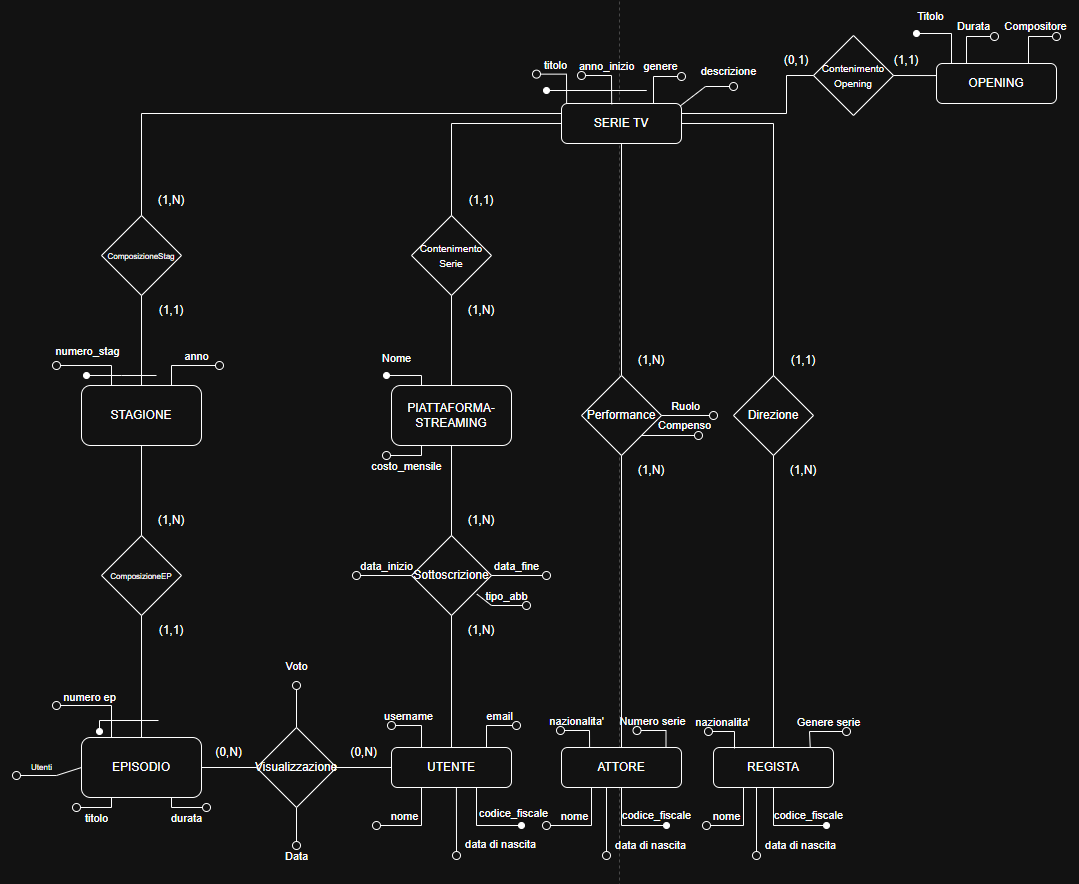
\includegraphics[scale=0.4]{schema-ristrutt.png}
    \caption{Schema E-R ristrutturato}
    \label{fig:ristrutt}
\end{figure}
% Aggiungi altre sezioni qui...
\subsection{Eliminazione delle generalizzazioni}
\textbf {Persona} è una generalizzazione totale di \textbf{UTENTE}, \textbf{ATTORE} e \textbf{REGISTA}, presenta
tre attributi \textit{Nome}, \textit{Data di nascita} e \textit{Identificatore}, ma non è legata a nessuna relazione.
Si nota quindi come questa generalizzazione possa essere eliminata. È preferibile infatti
accorpare i sue attributi nelle entità figlie. In questo modo si riduce il numero di attributi NULL rispetto all'operazione inversa,
ovvero accorpare gli attributi delle entità figlie in una sola entità padre.\newline
Inoltre, e' possibile eliminare l' attributo "codice\_fiscale" nell' entità "UTENTE" in quanto possiamo utilizzare l' attributo "username" come chiave primaria. Inoltre conoscere il codice fiscale di un utente puo' essere considerato sostanzialmente insensato e rischioso per la sicurezza.\newline
\textbf{In figura \ref{fig:ristrutt}} è riportato il diagramma E-R ristrutturato, in cui sono state effettuate le modifiche discusse precedentemente.

\subsection{Schema relazionale}
In seguito è riportato lo schema logico costruito a partire dallo schema E-R ristrutturato.
L'asterisco indica gli attrributi che possono essere NULL.
\begin{itemize}
    \item \textbf{Serie}(\underline{Titolo, AnnoInizio}, Genere, Descrizione, Regista, PiattaformaStreaming, Opening)
    \begin{itemize}
        \item Serie.Regista=Regista.CodiceFiscale
        \item Serie.PiattaformaStreaming=PiattaformaStreaming.Nome
    \end{itemize}
    \item \textbf{Stagione}(\underline{TitoloSerie, AnnoSerie, NumeroStagione}, Anno)
    \begin{itemize}
        \item Stagione.TitoloSerie=Serie.Titolo
        \item Stagione.AnnoSerie=Serie.AnnoInizio
    \end{itemize}
    \item \textbf{Episodio}(\underline{TitoloSerie, AnnoSerie, NumeroStagione, NumeroEpisodio}, Durata, Titolo)
    \begin{itemize}
        \item Episodio.TitoloSerie=Stagione.TitoloSerie
        \item Episodio.AnnoSerie=Stagione.AnnoSerie
        \item Episodio.NumeroStagione=Stagione.NumeroStagione
    \end{itemize}
    \item \textbf{Opening}(\underline{TitoloSerie, AnnoSerie}, Titolo, Compositore, Durata)
    \item \textbf{Visualizzazione}(\underline{Username, TitoloSerie, AnnoSerie, NumeroStagione, NumeroEpisodio}, Data, Voto*) 
    \begin{itemize}
        \item Visualizzazione.Username=Utente.Username
        \item Visualizzazione.TitoloSerie=Episodio.TitoloSerie
        \item Visualizzazione.AnnoSerie=Episodio.AnnoSerie
        \item Visualizzazione.NumeroStagione=Episodio.NumeroStagione
        \item Visualizzazione.NumeroEpisodio=Episodio.Numero
    \end{itemize}
    \item \textbf{Utente}(\underline{Username}, Nome, DataNascita, Email)
    \item \textbf{Attore}(\underline{CodiceFiscale}, Nome, DataNascita, Nazionalita, NumeroSerie)
    \item \textbf{Regista}(\underline{CodiceFiscale}, Nome, DataNascita, Nazionalita, GenereSerie)
    \item \textbf{PiattaformaStreaming}(\underline{Nome}, CostoMensile)
    \item \textbf{Sottoscrizione}(\underline{Username, Piattaforma}, DataInizio, DataFine*, TipoAbbonamento)
    \begin{itemize}
        \item Sottoscrizione.Username=Utente.Username
        \item Sottoscrizione.Piattaforma=PiattaformaStreaming.Nome
    \end{itemize}
    \item \textbf{Performance}(\underline{IDAttore, TitoloSerie, AnnoSerie}, Ruolo, Compenso)
    \begin{itemize}
        \item Performance.Attore=Attore.ID
        \item Perfomance.TitoloSerie=Serie.Titolo
        \item Performance.AnnoSerie=Serie.AnnoInizio
    \end{itemize}
\end{itemize}


\section{Implementazione in PostgreSQL e Definizione delle Query}

\subsection*{Definizione delle Query}

Di seguito vengono presentate e descritte le query con i relativi output generati e 
viene motivato l’utilizzo dell’indice proposto.

\vspace{1cm}

\subsubsection*{Query 1}
\textbf{Obiettivo:} Trovare tutti i titoli delle serie TV disponibili su una piattaforma specifica, ad esempio \textit{Netflix}.

\vspace{0.5cm}
\begin{center}
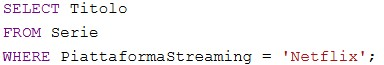
\includegraphics[width=0.9\textwidth]{Query1.jpg}
\end{center}


\begin{lstlisting}[caption={Esempio di query SQL}, label={lst:sql-example}]
SELECT name, genre
FROM tv_series
WHERE rating > 8.5
ORDER BY rating DESC;
\end{lstlisting}

\vspace{1cm}

\subsubsection*{Query 2 }
\textbf{Obiettivo:} Calcolare la media dei voti per ogni episodio della serie \textit{Dark}.

\vspace{0.5cm}
\begin{center}
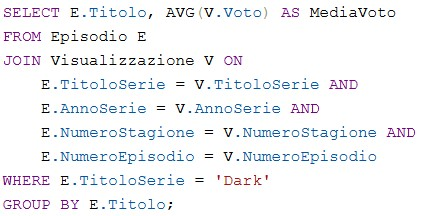
\includegraphics[width=0.9\textwidth]{Query2.jpg}
\end{center}

\vspace{1cm}

\subsubsection*{Query 3}
\textbf{Obiettivo:} Elencare gli utenti che hanno guardato almeno 5 episodi in totale.

\vspace{0.5cm}
\begin{center}
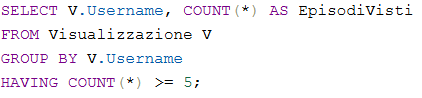
\includegraphics[width=0.9\textwidth]{Query3.png}
\end{center}

\vspace{1cm}

\subsubsection*{Query 4}
\textbf{Obiettivo:} Trovare gli attori che hanno recitato in almeno una serie vista dall’utente \texttt{mario\_rossi}.

\vspace{0.5cm}
\begin{center}
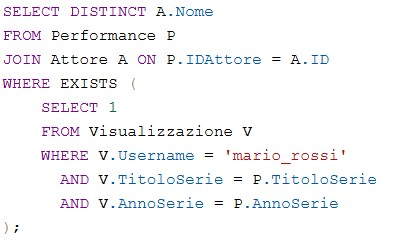
\includegraphics[width=0.9\textwidth]{Query4.jpg}
\end{center}

\vspace{1cm}

\subsubsection*{Query 5}
\textbf{Obiettivo:} Trovare le prime 3 serie TV (per numero totale di visualizzazioni) dirette da registi italiani e disponibili su piattaforme con costo mensile superiore a 10 euro.

\vspace{0.5cm}
\begin{center}
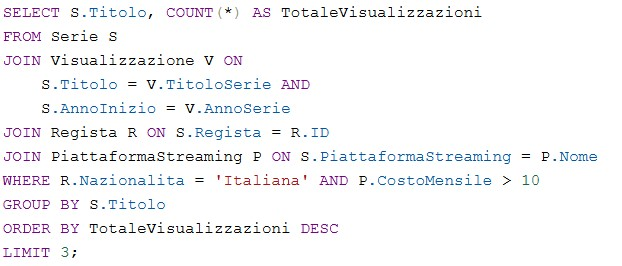
\includegraphics[width=0.9\textwidth]{Query5.jpg}
\end{center}

\vspace{1cm}

\end{document}
